\documentclass[twocolumn, 11pt]{article} % MÅ defineres i ethvert dokument.
\usepackage{longtable}
\usepackage{float}

\usepackage[utf8]{inputenc} %Tillater spesialteikn uten bruk av koding.
\usepackage[norsk]{babel} % Tillater norske teikn.
\usepackage[margin=1in]{geometry} % Definerer marger i dokumentet.
\usepackage{microtype} % Gjør det mer behagelig å lese dokumentet.
\usepackage{amsmath} % Tillater avansert formatering av matte.
\usepackage{amsfonts} % Tillater avanserte teikn, som R for reelle tall.
\usepackage[toc,page]{appendix} 
\usepackage{url}

\usepackage{tikz}
\usetikzlibrary{positioning}

\usepackage{graphicx} % Tillater mer avansert formatering av grafikk.
\usepackage{geometry} % Tillater enklere formatering av sidevisning.
\usepackage[colorlinks=true, pdfborder={0 0 0}]{hyperref} % Tillater hyperlenker {\href} som under. Colorlinks kan byttes til false hvis man ønsker linker i svart.
\usepackage[tableposition=top]{caption} % Tvinger tabelltekst til å dukke opp over alle tabeller.
\usepackage{graphicx}
\usepackage{float}
\graphicspath{ {./images/} }
\usepackage{listings}
\usepackage{color}
\definecolor{dkgreen}{rgb}{0,0.6,0}
\definecolor{gray}{rgb}{0.5,0.5,0.5}
\definecolor{mauve}{rgb}{0.58,0,0.82}
\lstset{frame=tb,
  language=Python,
  aboveskip=3mm,
  belowskip=3mm,
  showstringspaces=false,
  columns=flexible,
  basicstyle={\small\ttfamily},
  numbers=none,
  numberstyle=\tiny\color{gray},
  keywordstyle=\color{blue},
  commentstyle=\color{dkgreen},
  stringstyle=\color{mauve},
  breaklines=true,
  breakatwhitespace=true,
  tabsize=1
}
\begin{document}

\twocolumn[
  \begin{@twocolumnfalse}
\textbf{
  \title{Spektralanalyse av alger og sirup ved UV/vis-spektroskopi}
  \author{Bård Tollef Pedersen og Erik Lykke Trier}
  \date{22. januar 2023} % \today gir dagens dato
  \maketitle
}
    \begin{abstract}
    \begin{large}
    \
    Denne rapporten tar for seg spektroskopi av alger og fargede siruper. Formålet er å se om man kan gruppere stoffene ved hjelp av på spektroskopi. 
    Resultatet viser at det gir best gruppering med PCA uten forbehandling, hvor blå og indigo er de mest vektete områdene i spekteret. Når man ser på bølgetall mot absorpsjon for alle forsøkene så blir dataene samlet ved lave bølgetall og utstrakt ved høye bølgetall. 
    
    
    \end{large}
    \end{abstract}
  \end{@twocolumnfalse}     
  ]
\section{Innledning} 


Spektroskopi en uendelighet av molekyler og elektromagnetisk stråling. Ingen vet hvor mange kombinasjoner det er av lyskilder og stoffer som kan absorbere og reflektere forskjellige lysstråler. Når elektromagnetisk stråling passerer gjennom et stoff blir deler av strålingen absorbert, deler vil passere rett gjennom og andre deler vil reflekteres. Her testes det om hvilke deler av strålingen som blir absorbert av alge og farge sirup prøvene ved hjelp av et spektrometer. 

I dette forsøket er det brukt spektroskopi på forskjellige siruper og alger. Formålet er å se om man kan skille de forskjellige stoffene med urenhetene i ved hjelp av spektroskopi. Det skal brukes spektrometer og Quasar til  å samle inn og behandle data. Ved hjelp av PCA skal det undersøkes om man kan gruppere prøvene ved å gjennomføre PCA.





\section{Teori og metoder}

\subsection{Spektroskopi}
Spektroskopi er en rekke metoder for å studere atomer og molekyler. Dette gjøres ved å måle bølgelengder emittert eller absorbert fra det observerte legeme\cite{spektroskopi}, der bølgelengde er avstanden mellom to like punkter i en bølge, ofte mellom toppunkt eller bunnpunkt\cite{taylor1997error}.

I tilleg til bølgelengde brukes også bølgetall som en forklaring i dette forsøket. Formelen for å gjøre om fra bølgelengde til bølgetall er gitt med formel \eqref{Bølgetall}.

\begin{equation}
    \bar{\nu} = \frac{1}{\lambda}
    \label{Bølgetall}
\end{equation}

Henviser til \eqref{Bølgetall}, der \textit{$\bar{\nu}$} er bølgetall, \textit{$\lambda$} er bølgelengde, begge oppgitt i \textit{cm}

\bigskip

I dette forsøket blir det benyttet et UV-spektroskopi. UV-spektroskopi er et måleinstrument som baserer seg på atomer og molekyler sin evne til å absorbere eller emittere ultrafiolett stråling. Mer nøyaktig benyttes det et UV-vis spektroskopi. Dette spektrometeret måler hovedsaklig det synlige lyset. 

Spektrometer modellen som blir brukt er en \textit{PASCO wireless transmittance}. Dette spektrometer har en enhetsfeil på $\pm$ 2.5 nm \cite{oppgavetekst}.

Dette spektrometeret brukes sammen med dets egne programvare. Programmet kobles til spektrometeret via enten \textit{Bluetooth} eller \textit{USB}. Programmet gjør det lett å visualisere bølgelengdene med absorpsjonsverdiene, disse dataene kan så bli lagret som csv filer. I programmet kan en også justere på 2 parametere, antall målinger for gjennomsnitt og glatting. Glatting ble satt på 25 og antall målinger for gjennomsnitt ble også satt til 25. 

\subsection{PCA og forbehandlinger}
PCA eller hovedkomponentanalyse er en metode for å transformere et sett med observasjoner av mulig korrelerte variabler til et sett med observasjoner av uavhengige variabler kalt hovedkomponenter. Det gjør dette ved å finne de linjene i datarommet som har maksimal variasjonsdekning. Hovedkomponentene er lineært uavhengige av hverandre og er ordnet slik at den første hovedkomponenten har mest mulig variasjonsdekning\cite{youtube}.

For å få best mulig gruppering er det testet både med og uten forbehandlinger. De forbehandlingene som ble benyttet er EMSC og Savitzky-Golay.  
Utvidet multiplikativt signal korreksjon (EMSC) er en metode for å korrigere for skjevheter i spektroskopiske data. Denne metoden er ofte brukt for å forbedre nøyaktigheten og påliteligheten av spektroskopiske data\cite{oppgavetekst}.

Savitzky-Golay algoritmen er en metode for å filtrere eller glatte ut data. Denne algoritmen er ofte brukt for å fjerne støy eller andre uønskede variasjoner i signalene\cite{oppgavetekst}.


\subsection{Alger og farger}
Alger en en gruppe av ulike encellede og flercellede organismer, hvor fellesbetegnelsen er at de lever fuktig og benytter seg av fotosyntese \cite{Alger}. I dette forsøke ble algene i tabell \ref{table:1} benyttet. I tabell \ref{table:1} kan en se både det vitenskapelige navnet på algen samt en forkortelse som blir benyttet i denne rapporten.

\begin{table}[H]
\begin{tabular}{|c|c|} 
\hline
Vitenskaplig navn & Forkortesle \\
\hline
\textit{Chlorella vulgaris} & CVU \\
\textit{Botryococcus Braunii} & BBR\\ 
\textit{Vischeria polyphem} & VPO \\ 
\textit{Neochloris oleoabundans} & NOL \\
\textit{Scenedesmus sp} & SSP\\
\hline
\end{tabular}
\caption{Vitenskaplig navn på alger med de representative forkortelsene.}
\label{table:1}
\end{table}


Det ble også målte fortynnede prøver av algene. Første fortynning ble det fjernet ca 1/3 av innholdet i test-røret for så å fylle det oppigjen med vann. Andre fortynning ble det igjen fjernet ca 1/3 av den allerede fortynnede blandingen og fylte oppigjen med vann. Total ble det 3 grader av fortynninger per alge, ufortynnet, litt fortynnet og veldig fortynnet.

I tilleg til alger ble det også benyttet fargede sirup. Det ble brukt tre farger i forskjellige blandinger, rød, gul og blå. De forskjellige blandingene av farger kan sees i tabell \ref{Simplex Lattice Design}. 

\begin{table}[H]
\centering
 \begin{tabular}{||c c c||} 
 \hline
 Rød & Blå & Gul\\ [0.5ex] 
 \hline\hline
 1 & 0 & 0 \\
 0.66 & 0.33 & 0 \\
 0.33 & 0.66 & 0 \\
  0 & 1 & 0 \\
 0 & 0.66 & 0.33 \\
 0 & 0.33 & 0.66 \\
 0 & 0 & 1 \\
 0.33 & 0 & 0.66 \\
 0.66 & 0 & 0.33 \\ 
 0.33 & 0.33 & 0.33 \\[1ex] 
 \hline
 \end{tabular}
 \caption{Blandingsforholdet mellom rød, blå og gul for å lage de ti forskjellige målingene som ble brukt.}
 \label{Simplex Lattice Design}
\end{table}


Det ble tatt tre målinger av alle prøvene. Så totalt ble det tatt 45 målinger av algene og 30 målinger av fargene. 

\subsection{Orange/Quasar}
Orange er et verktøy for maskinlæring og visualisere data. Dette gjør at kvalitativ dataanalyse og datavisualisering enkelt og raskt kan gjennomføres\cite{Orange}.

Quasar er en utvidet version av Orange-pakken. Denne utvidelsen gjør det enkelt å gjennomføre PCA og spredningsplot\cite{Quasar}.

\bigskip

Quasar ble brukt for å plotte spektre, PCA og ladningsplott. For at Quasar skulle kunne lese og jobbe med dataen måtte dataen først lagres som csv fil fra programvaren til spektrometeret, for så å bli bearbeidet i Excel. Excel er et program for å lagre, redigere og analysere data i tabeller.
I Excel ble alle kollonene med emittering verdier fjernet, ettersom bare absorpsjon skal analyseres. Deretter ble kollonene transponert så kollonene ble til rader. 
For at Quasar skal kunne automatisk gjenkjenne kategoriske og numeriske variabler ble også alle tall formert med tre desimaler. Deretter ble det lagt til variabel navn for å lettere skille og analysere data i plottene. Det ble lagt til en kolonne for alge type, utvanning av alger og farge.
Excel ble også brukt for å gjøre om bølgelengde til bølgetall ved hjelp av formel \eqref{Bølgetall}.


\section{Resultater}

Når en skal skille to eller flere spektra fra hverandre kan det hjelpe å endre fra bølgelengde til bølgetall. I figur \ref{alger_lengde} kan en se spekteret til de forskjellige algene plottet med bølgelengde og i figur \ref{alger_tall} kan en se 
det samme spekteret som i figur \ref{alger_lengde}, men plottet med bølgetall.  Her er absorpsjonen plottet som y-aksen, hvor tallene mellom 0 og 3 representerer 0\% til 100\% absorpsjon. I figur \ref{farge_lengde} og \ref{farge_tall} kan en se spekteret til tre farger, rød, gul og blå. Her viser figur \ref{farge_lengde} spekteret plottet med bølgelengde og figur \ref{farge_tall} viser bøletall. I disse plottene kan en se at bølgetall strekker lave bølgelengder og kompromerer høye bølgelengder.

 
\begin{figure}[H]
\includegraphics[width=0.5\textwidth]{Lab3/Images/bølgelengde.png}
\caption{Absorpsjon plottet med bølgelengd for de forskjellige alge typene.}
\label{alger_lengde}
\end{figure}

\begin{figure}[H]
\includegraphics[width=0.5\textwidth]{Lab3/Images/bølgetall.png}
\caption{Absorpsjon plottet med bølgetall for de forskjellige alge typene}
\label{alger_tall}
\end{figure}

\begin{figure}[H]
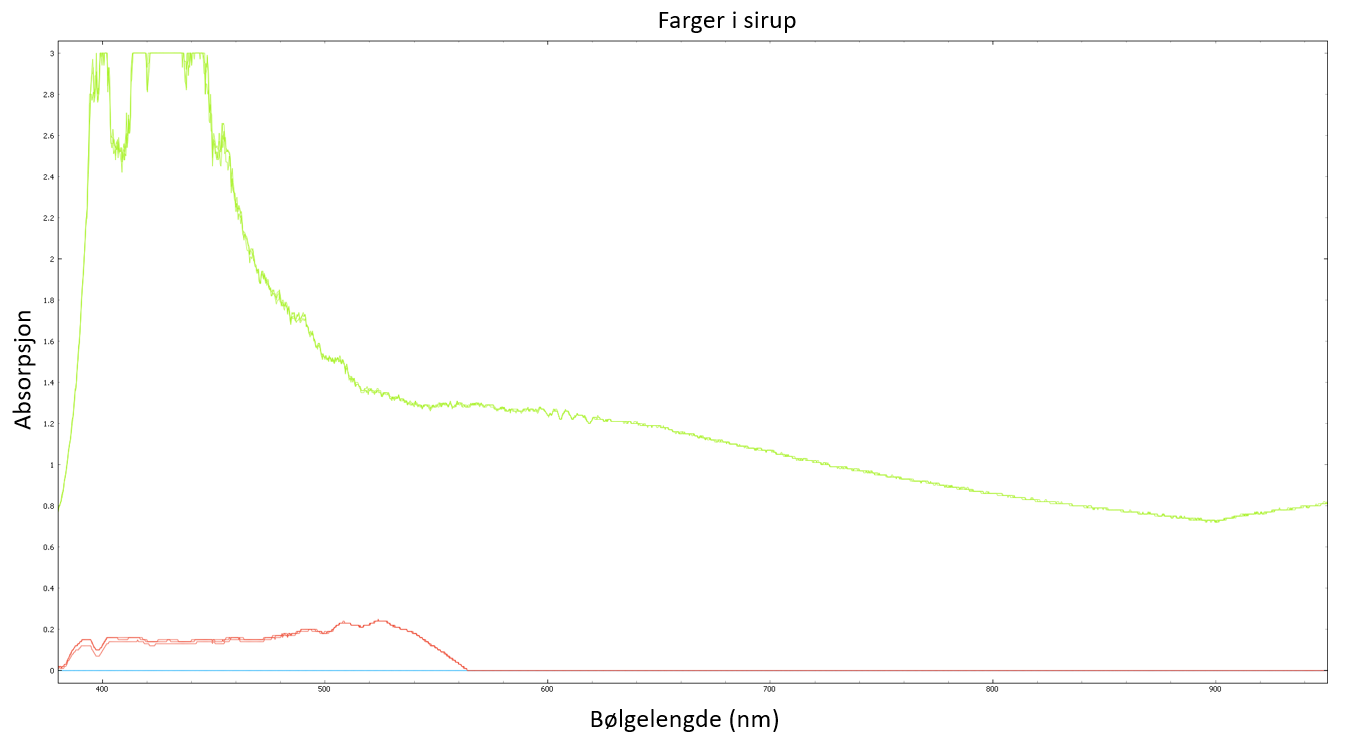
\includegraphics[width=0.5\textwidth]{Lab3/Images/sirupVSlengde.png}
\caption{Absorpsjon plottet med bølgelengde for de forskjellige fargene.}
\label{farge_lengde}
\end{figure}

\begin{figure}[H]
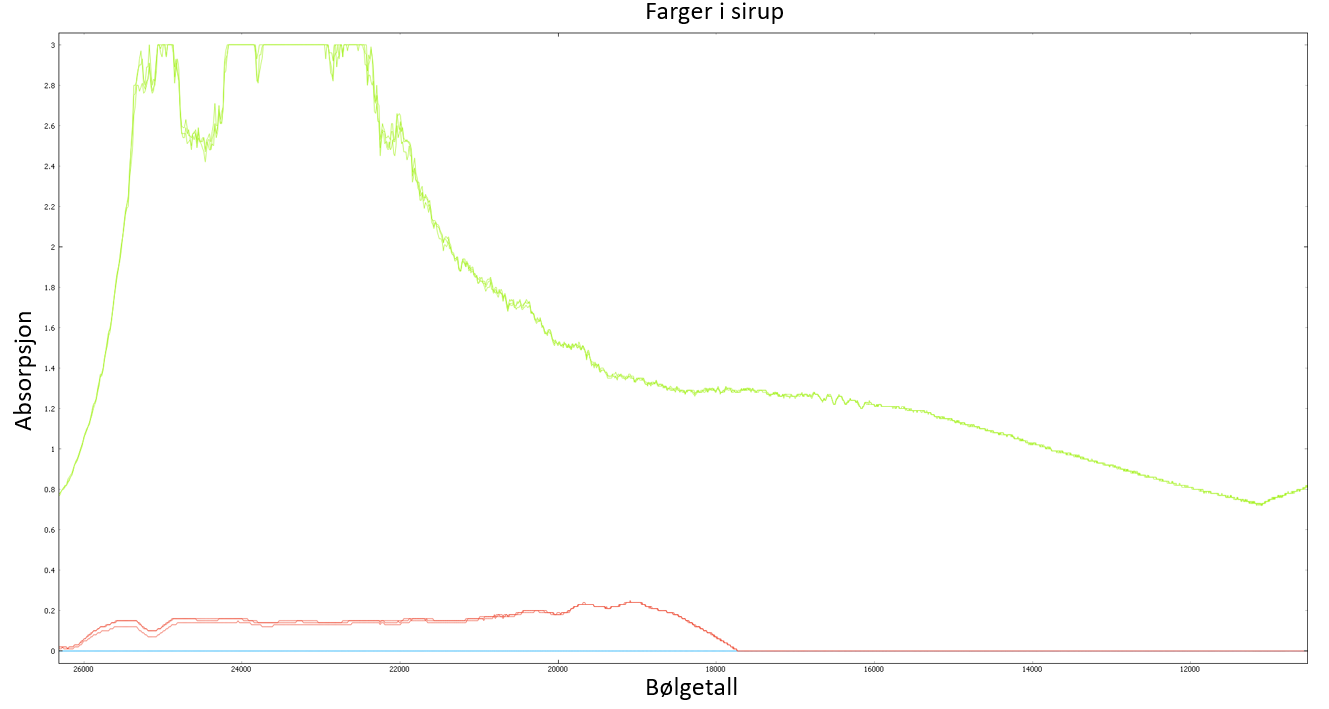
\includegraphics[width=0.5\textwidth]{Lab3/Images/sirupVStall.png}
\caption{Absorpsjon plottet med bølgetall for de forskjellige fargene.}
\label{farge_tall}
\end{figure}


\newpage
For å finne best mulige gruppering er det testet med forskjellige forbehandlinger. De forbehandlingene det ble testet gruppering med er EMSC og Savitzky-Golay. Grupperingene som ble sett på var mellom de forskjellige algene og de forskjellige fortynninger av alger. Totalt er det fire forskjellige PCA plott som viser grupperingene med de forskjellige forbehandlingene. I figur \ref{PCA_alger} er det ikke brukt noen forbehandlinger. Her kan en se at det er grupperinger mellom algene og når algene blir fortynnet blir også grupperingene mer samlet på tvers av algetypene. I figur \ref{PCA_alger_EMSC} er det brukt EMSC som forbehandling. Her kan en se at BBR er tydelig gruppert fra resten. Her kan en også se at det er litt dårligere gruppering enn figur \ref{PCA_alger}.
I figur \ref{PCA_alger_Savi} er der brukt Savitzky-Golay som forbehandling, her kan en se at CVU og NOL uten fortynning har tydelige grupperinger utenfor resten. Men grupperingene på de andre er dårligere. I den siste figuren, figur \ref{PCA_alger_EMSC_Savi} er det både brukt EMSC og Savitzky-Golay som forbehandlinger. Her kan en se at BBR er over alt på plottet, mens resten av prøvene er samlet rundt null.

\begin{figure}[H]
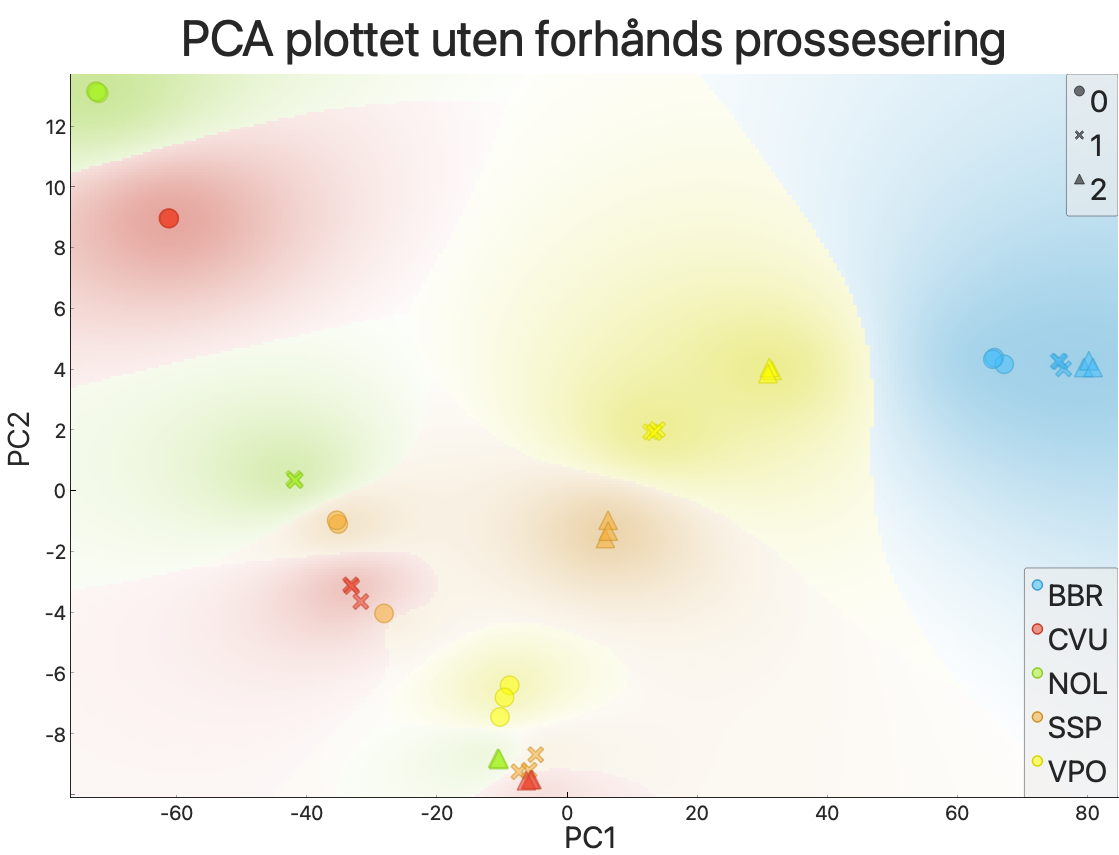
\includegraphics[width=0.5\textwidth]{Lab3/Images/PCA_Uten.png}
\caption{PCA av alger med fortynning plottet uten forprosess. Der farger skiller de forskjellige algene og form skiller de forskjelle fortyningene, der 0 er ufortynnet og 2 er veldig fortynnet.}
\label{PCA_alger}
\end{figure}


\begin{figure}[H]
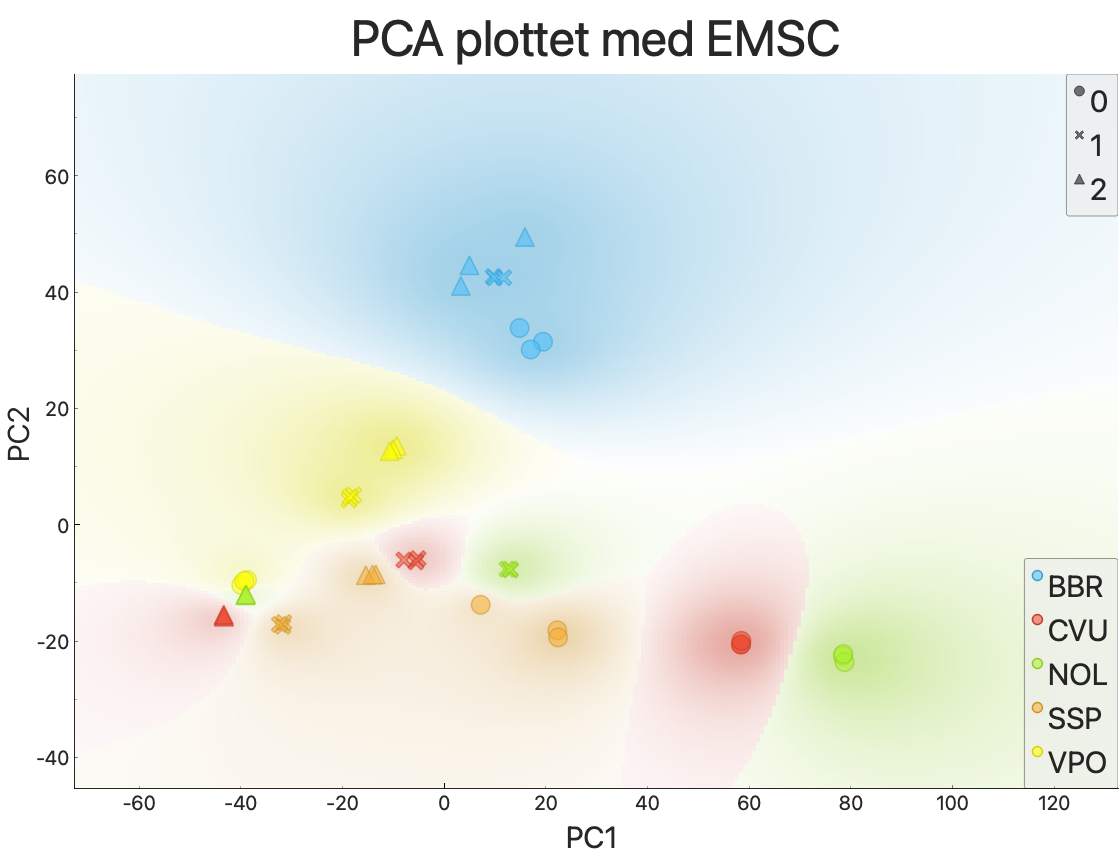
\includegraphics[width=0.5\textwidth]{Lab3/Images/PCA_EMSC.png}
\caption{PCA av alger med fortynning plottet med EMSC som forprosess. Der farger skiller de forskjellige algene og form skiller de forskjelle fortyningene, der 0 er ufortynnet og 2 er veldig fortynnet}
\label{PCA_alger_EMSC}
\end{figure}

\begin{figure}[H]
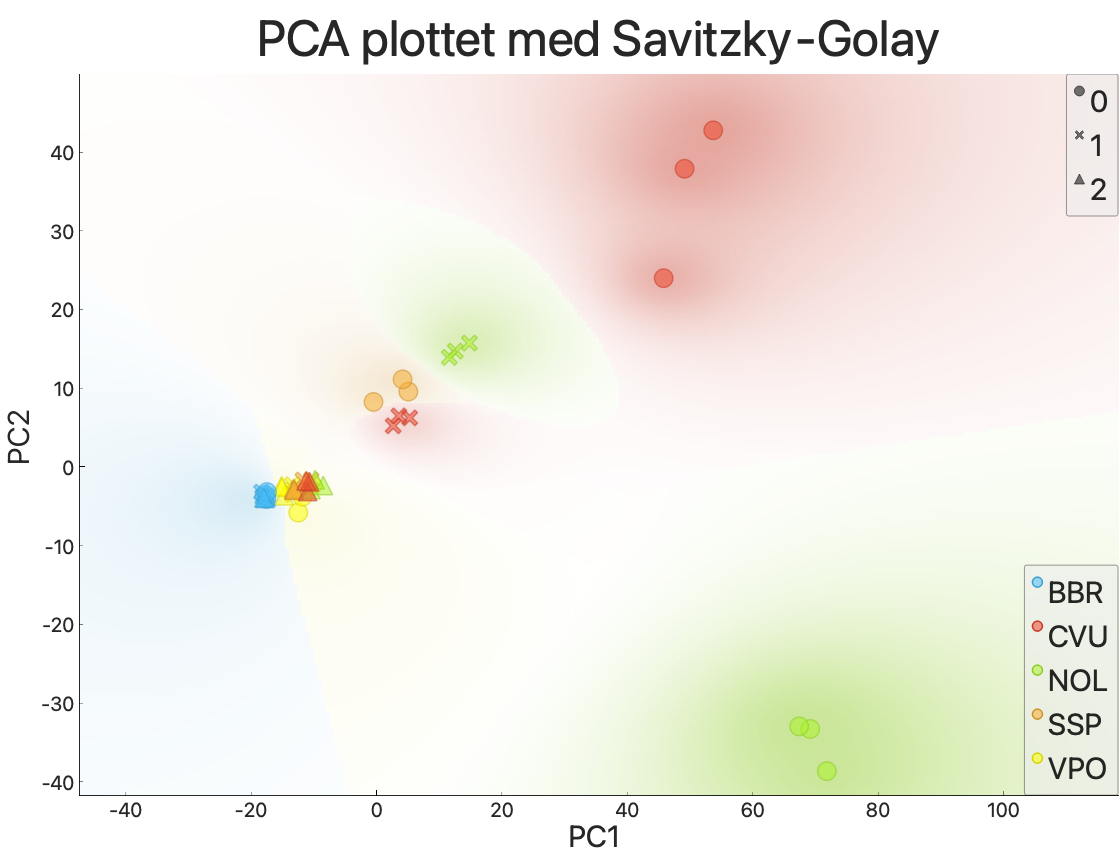
\includegraphics[width=0.5\textwidth]{Lab3/Images/PCA_Savitzky.png}
\caption{PCA av alger med fortynning plottet med Savitzky-Golay som forprosess. Der farger skiller de forskjellige algene og form skiller de forskjelle fortyningene, der 0 er ufortynnet og 2 er veldig fortynnet}
\label{PCA_alger_Savi}
\end{figure}

\begin{figure}[H]
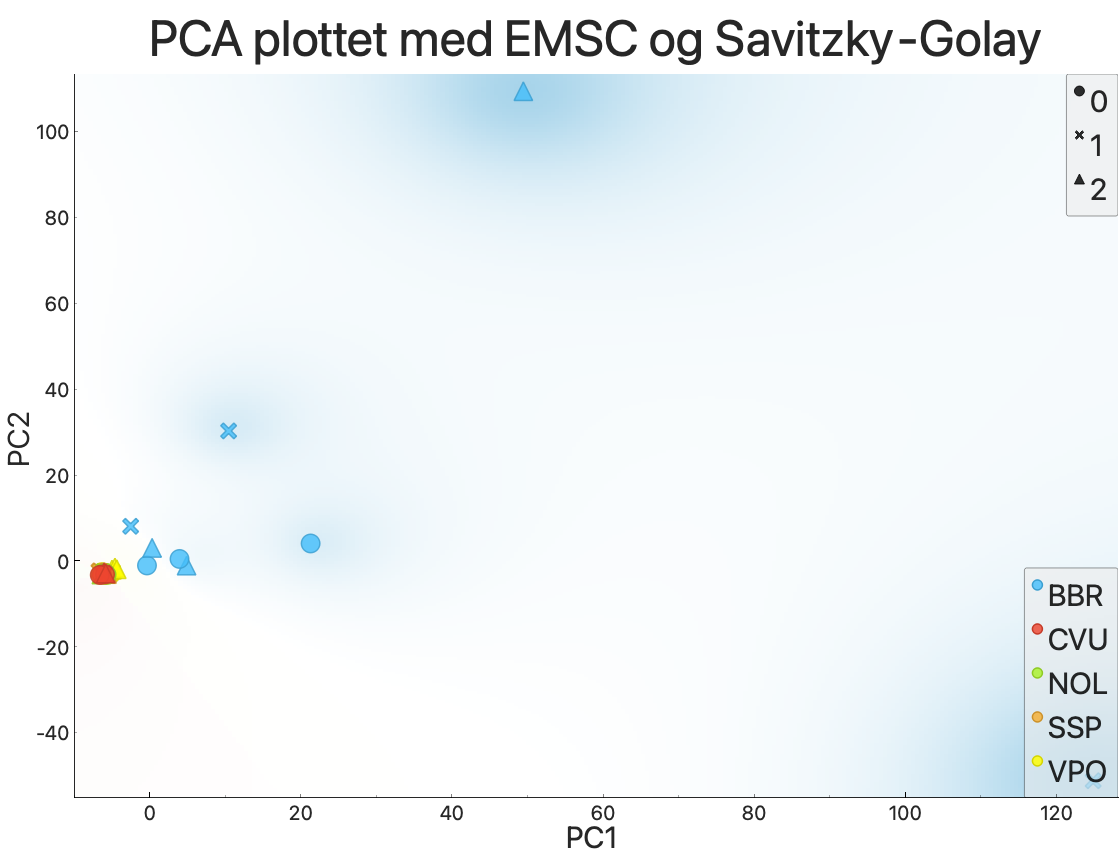
\includegraphics[width=0.5\textwidth]{Lab3/Images/PCA_EMSC_Savitzky.png}
\caption{PCA av alger med fortynning plottet med EMSC og Savitzky-Golay som forprosess. Der farger skiller de forskjellige algene og form skiller de forskjelle fortyningene, der 0 er ufortynnet og 2 er veldig fortynnet}
\label{PCA_alger_EMSC_Savi}
\end{figure}


Når en ser på PCA ser en at farger og alger gruppere seg. For å se hvilke bølgelengder som skiller de forskjelle gruppene kan en se på ladningsplottet. Det er det en kan se i figur \ref{farge_ladningsplott} og \ref{alger_ladningsplott}. I figur \ref{farge_ladningsplott} kan en se ladningsplottet til figur \ref{farge_pca}. Der figur \ref{farge_pca} er en PCA av de forskjellige fargene og blandingene fra tabell \ref{Simplex Lattice Design}. Her kan en se at pc1, den blå grafen, har bølgelengder rundt 450 til 550 nm med høyest verdi. Kan også se at pc2 holder seg jevn over hele spekteret 

I figur \ref{alger_ladningsplott} kan en se ladningsplottet til figur \ref{PCA_alger}. Her kan en se at første hovedkomponenten blir vektet mye av bølgelengder mellom 390 til 425 nm. Kan også se at det er jevne verdier fra 500 nm til 900 nm. Her kan en se at pc2 også holder seg jevn akkurat som i figur \ref{farge_ladningsplott}.


\begin{figure}[H]
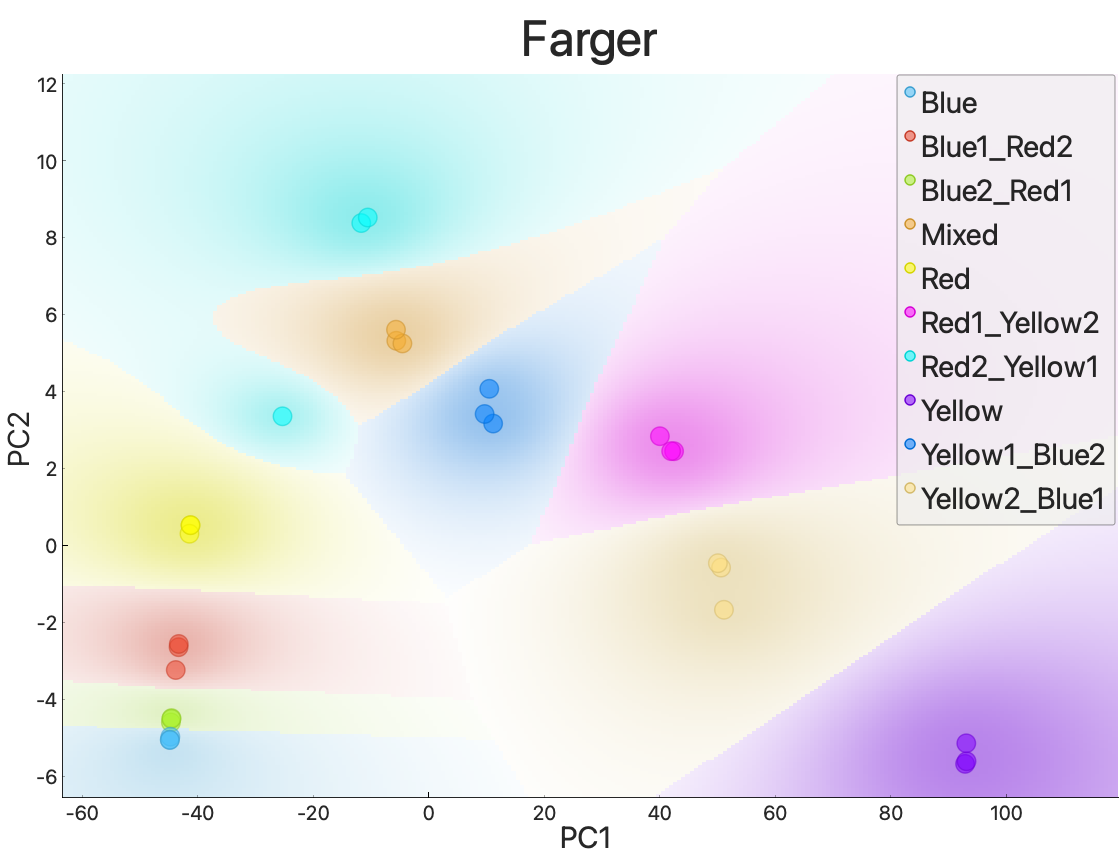
\includegraphics[width=0.5\textwidth]{Lab3/Images/Farger_alle_PCA.png}
\caption{Farger og farge blandinger plottet med pc1 og pc2.}
\label{farge_pca}
\end{figure}

\begin{figure}[H]
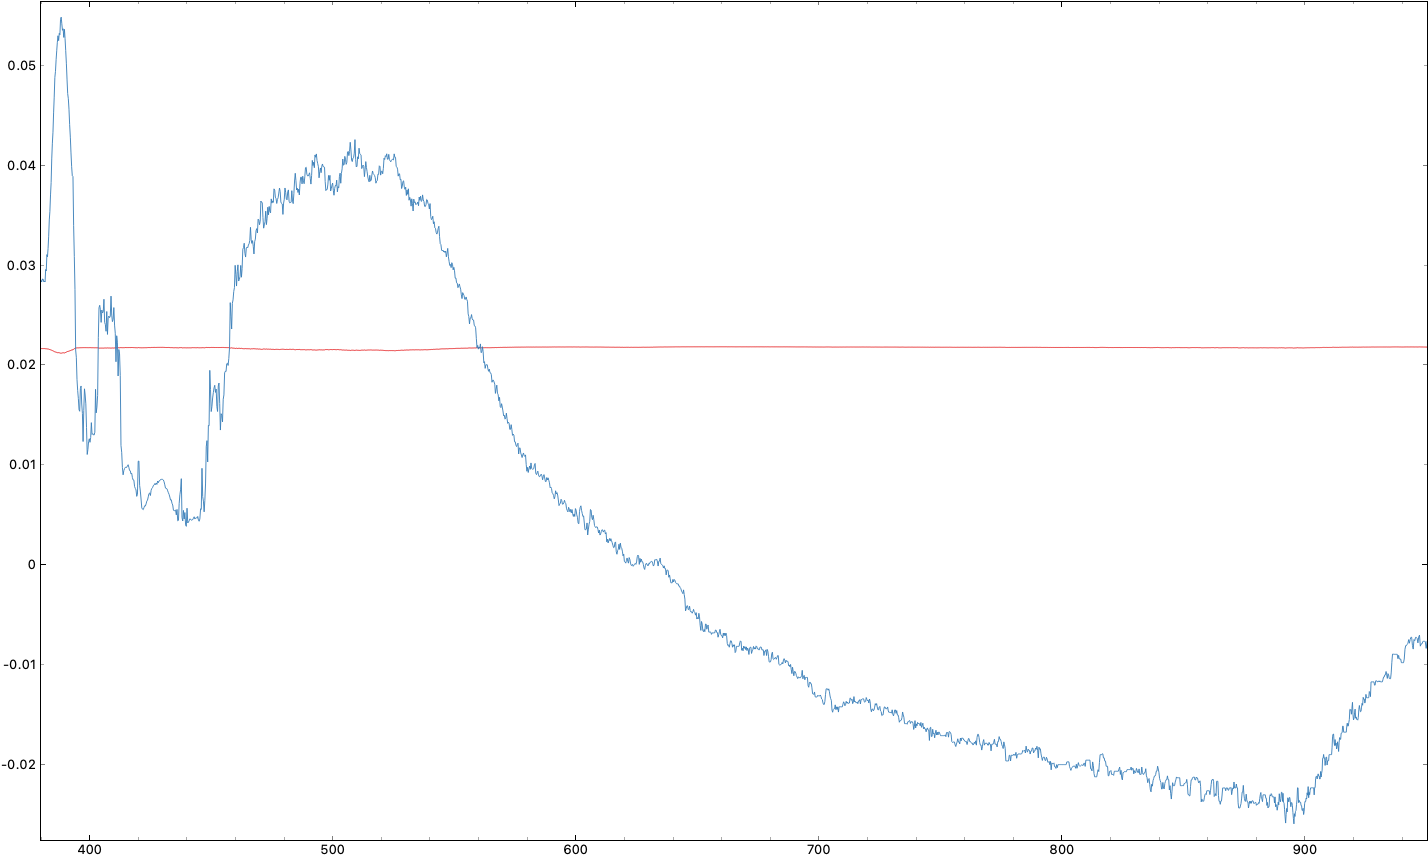
\includegraphics[width=0.5\textwidth]{Lab3/Images/Farger_Alle_Ladningsplott.png}
\caption{Ladningsplottet til PCA av farge analysene, hvor x-aksen er bølgelengde (nm), og y-aksen er hvor mye bølgelengden vektes av hovedkomponenten. Blå linje er pc1 og rød line er pc2.}
\label{farge_ladningsplott}
\end{figure}


\begin{figure}[H]
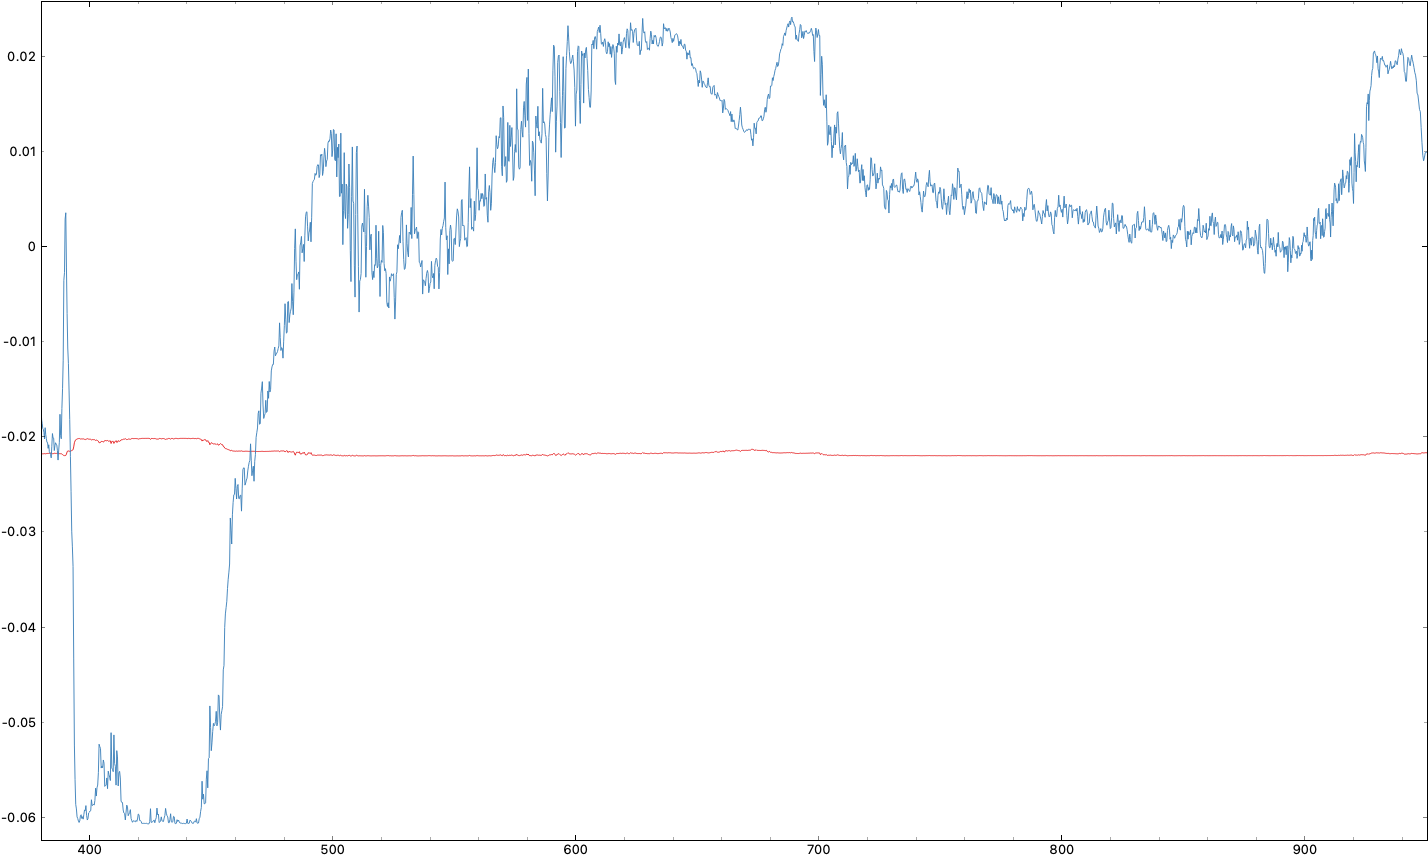
\includegraphics[width=0.5\textwidth]{Lab3/Images/Alger_alle_ladningsplott.png}
\caption{Ladningsplottet til PCA av alge analysene, hvor x-aksen er bølgelengde (nm), og y-aksen er hvor mye bølgelengden vektes av hovedkomponenten. Blå linje er pc1 og rød line er pc2.}
\label{alger_ladningsplott}
\end{figure}

\section{Diskusjon}
Hvis en ser på figur \ref{alger_lengde}, \ref{alger_tall}, \ref{farge_lengde} og \ref{farge_tall} kan en se at bølgetall endrer litt på plottet. Det en kan se fra plottene er at bølgetall strekker spektrene i de lave bølgelengdene og kompromerer i de høye. Dette gjør at en lettere kan se forskjell på data i lave bølgelengder ved å plotte med bølgetall. Det vil også gjøre det vanskeligere å se forskjell på data i høye bølgelengder. 
Når en kun ser på de tre hoved fargene eller algene uten noen fortynninger er det ikke mye hjelp å få ved å endre fra bølgelengde til bølgetall. Dette er fordi det allerede er stor forskjell, det er også forskjell jevnt over, så det å strekke eller kompromere spektre vil ikke gi noen fordel eller ulempe.  

\bigskip
I figur \ref{PCA_alger_EMSC} og \ref{PCA_alger_Savi} kan en se grupperinger. I figur \ref{PCA_alger_EMSC} kan en lett skille ut BBR. En kan også se grupperinger blant de andre algene, men de er mye nærmere hverandre. I figur  \ref{PCA_alger_Savi} kan en lett skille ut CVU, her er det også en gruppering med ufortynnet NOL som er langt unna de andre gruppene. Uten om det er det en stor samling av alger, både fortynnet og ufortynnet rundt null.
på figur \ref{PCA_alger_EMSC_Savi} er det elendig grupperinger og fordelinger. Alle prøvene er samlet på omtrent null. Det er noen uteliggere av BBR, dette er også den algen som skiller seg mest ut. 

Fra de forskjellige PCA plottene, figur \ref{PCA_alger}, \ref{PCA_alger_EMSC}, \ref{PCA_alger_Savi} og \ref{PCA_alger_EMSC_Savi} kan en se at mer prosessert data gir dårligere gruppering. En av grunnene til dette kan være at det ikke er så stor forskjell mellom de. Så den lille forskjellen mellom algene blir borte når en prosesserer data. 

\bigskip


I figur \ref{farge_pca} og \ref{farge_ladningsplott} kan en se PCA og ladningsplottet til fargene. Her kan en se at det er en god gruppering. Eneste som ligger litt utenfor gruppen sin er en av målingene til blandingen av to deler rødt og en del gult. Her er to målinger samlet og den tredje litt utenfor, det kan være fler grunner til dette. En av de er om den ikke var godt nok blandet første gang. Når den ble flyttet og løftet på kan den ha blitt bedre blandet. Dette ville gjort at første målingen ligger litt utenfor. Det kan også hende at det har kommet fingeravtrykk på siden av test-røret som ville gjort at siste målingen ville ligget utenfor.

Fra figur \ref{farge_ladningsplott} kan en se at det som vektes mest i pc1 er spekteret mellom 450 og 550 nm. Dette spekteret tilsvarer det blå lyset. En kan også se en topp rundt 380 til 400 nm, som tilsvarer det fiolette lyset. Det er veldig lite rundt 610 til 625 nm, som tilsvarer det oransje lyset. Dette vil si at det oransje lyset nesten ikke blir brukt for å skille de forskjellige gruppene, mens blå og indigo er veldig vektet når det kommer til grupperingene. På pc2 er det veldig jevnt med en varians på 0.02 gjennom hele spekteret. Det vil si at alle farger og bølgelengder blir like mye vektet i grupperingen.


I figur \ref{PCA_alger}, \ref{alger_ladningsplott} kan en se PCA og ladningsplottet til alle algene med tre nivåer av fortynning. På spredningsplottet eller figur \ref{PCA_alger} kan en lett se grupperinger. Det er tydeligst gruppering med prøvene uten fortynning, men dette er også forventet ettersom det er mer konsentrert med prøvene og forskjellene blir derfor også tydeligere. En kan også se et BBR algene er lettest å gruppere. De er lengst til høyre i plottet og alle prøvene, selv de fortynnede er samlet. 

Det er en tydelig uteligger med SSP, dette kan være samme grunnen som uteliggeren i spredningsplottet til fargene. Enten at det har kommet møkk på test-røret eller at den ikke er blandet bra nok. Ettersom det er ren alge og ikke noe fortynning kan man tenke seg at det har kommet møkk på test-røret. 
Det er en liten samling med blanding nederst i midten, de fleste av disse er fortynnet. Dette er som forventet ettersom fortynnede prøver gir svakere absorpsjon og det blir vanskeligere å skille

Hvis en ser på \ref{alger_ladningsplott} kan en se at pc1 er mest vektet i området 390 til 425 nm, dette tilsvarer fargen indigo. 
En kan også se at det er nesten ikke noe forklaring fra 470 nm, men ganske jevnt fra 500 nm til 900 nm. Noe som vil si at mye av vektingen ligger i indigo spekteret og resten av spekteret utenom det blå lyset.

Det samme kan en se på pc2 her som i pc2 i figur \ref{farge_ladningsplott}. En jevnt verdi på 0.02 gjennom hele spekteret. Som vil si at alle farger og bølgelengder blir omtrent like mye vektet.


\bigskip 

Som nevnt kan en av feilkildene være dårlig rørt og blandet av prøvene. Dette vil gjøre at man ikke får optimale målinger.
En annen feilkilde er fingeravtrykk på rør. Dette gjør at man målet bakterier og stoffer som har vært på fingeren din og ikke prøven. Det samme kan skje om prøve-glassene ikke var godt nok rengjort før forsøk.

Noe annet som kan påvirke dataen er dårlig kalibrering av spektrometeret, eller for mye utjevning i \textit{PASCO's Spectrometry} programmet. For mye utjevning gjør at man mister data som kunne hjulpet med å lettere gruppere prøvene.


\section{Konklusjon}

Bølgetall gjør at det blir strekt med lave bølgelengder og komprimert med høye bølgelengder. Dette hjelper ikke med å gruppere farger eller alger i dette forskøket. Ingen forbehandlinger gir best grupperinger på PCA blant algene, ettersom man fjerner for mye data som skiller algene med forbehandlinger. Tilslutt så gir PCA  gode grupperinger med ufortynnede alger. PCA gir helt greie grupperinger i farger, men det er vanskelig å skille blandinger med blå og rød. Det er også vanskelig å skille de fortynnede prøvene av alger.

\bibliographystyle{plain}
\bibliography{sources3.bib}

\end{document}

